\documentclass[]{article}
%\documentclass[twocolumn]{article}
% \usepackage[backend=bibtex,style=verbose-trad2]{biblatex}
\usepackage[utf8]{inputenc}
\usepackage[english]{babel}
\usepackage{graphicx}

%opening
\title{Ternary Augmented Raft Architecture}
\author{Ganesh Prasad Kumble}

\begin{document}

\date{}
\maketitle

\begin{abstract}
This paper presents a new consensus algorithm based on Byzantine Fault Tolerant\cite{ARTICLE:1} RAFT \cite{ARTICLE:2} with a hybrid architecture framework that proposes linear as well as exponential robustness in the back-end systems supporting various sorts of transactions that demand absolute speed, resilience, accuracy, integrity and trust.
\end{abstract}

\section{Background}
Distributed systems have become quintessential in empowering the digital growth of organizations in many verticals. It is a shared responsibility among ourselves to simplify and yet provide architecture that can exhibit stable properties and support financial or commodity transactions from multiple verticals that demand a trusted environment. Readers are highly encouraged to go through the cited articles on PBFT \cite{ARTICLE:1}, RAFT \cite{ARTICLE:2}, and Tangaroa \cite{ARTICLE:3} thoroughly before reviewing this paper.

\section{Introduction}
The TARA architecture leverages a compound set of theories such as Practical Byzantine Fault Tolerance\cite{ARTICLE:1}, Raft Algorithm\cite{ARTICLE:2}, and cryptographic message exchange etc. on top of the distributed systems\cite{ARTICLE:3}. Each concept derived from the above is effectively combined to form an architecture that serves the core purpose of laying out a stable architecture to transact, manage and represent relevant transactions of a commodity.

\subsection{Grand Nodes}
Grand nodes are independent group of nodes distributed across the geography to perform as gatekeepers.
Gatekeeping activities include the reception of incoming messages, transaction payloads, and classify them based on the relevant asset class tagged.
Grand nodes are dedicated resources that have above the par computational power to perform gatekeeping activities in a reliable manner. Nodes with a dedicated amount of computational hardware, NTQ and stake can participate as a candidate to be elected as one of the grand node.

\subsection{Star Nodes}
Star nodes are the federated leaders of a small cluster with size ranging from a minimum of 4 nodes and above.
The duty of a Star Nodes is to recieve the set of transactions grouped by grand nodes into respective asset class and perform formal verification of these transactions.
The formally verified transactions are now bundled into a new block based on the timestamp proximity and propogated across other clusters in the network. 

\subsection{Service Nodes}
Service Nodes are the followers in the cluster, and recieve the asset-specific transactions of interest from their leader Star Node and perform formal verification. Majority of the service nodes are expected to pass the formal verification by default to propogate a block. However, platforms can be given the freedom and flexibility to customize the same intenrally on a case-by-case basis.

\subsection{Service Cluster}
The service clusters provides response-oriented functionality upon client request. Hence, each node representing a service node may contain service logic and service content to be delivered upon the client request. Each service cluster consists of a leader called “A mode” node or “V mode” node based on the nature of the leader in the term. If the leader is performing an output transaction (TX), then it behaves as an V mode node. Else, if the leader is performing an input transaction (RX), then it behaves as a A node. As mentioned in the Raft Algorithm\cite{ARTICLE:2}, the leader node broadcasts the received message or transaction to its followers in the current term to commit them into respective logs and checks the ‘nextIndex’ value to determine its nature of operation for the next term. For the sake of simple explanation, we observe the leader to be in either one of the mode. However, the system prescribes to the concept of multi-processing since modern computers are able to equip hybrid nature. If a leader fails to manage the transaction log, a new election shall take place as mentioned in the Raft algorithm\cite{ARTICLE:2}.

\subsection{Basic Network}
The TARA architecture comprises of modular components that are supported by the theory of Practical Byzantine Fault Tolerance[1]. As the name of the proposed architecture suggests, each service cluster shall comprise of exactly 3 nodes. The reason for the cardinality of nodes shall be explained further in accordance to the concept of byzantine failures. A minimum of 2 service clusters are connected to each other in the form of a distributed bus, connected via an interconnect node called “star node”, hence forming a basic operational case of seven nodes in a distributed environment. The star node is a randomly elected leader as per the election rules of Raft Algorithm[2], more elaborated in further sections.

\section{Algorithm}
\subsection{Federated leadership}
\subsection{Message passing}
\subsection{Log replication and consensus}
\subsection{Follow-up Sync}

\section{Correctness}
The novel aspect of the TARA architecture can be observed by considering the failure scenario mentioned above. A TARA distributed network suffering from 2 byzantine faults in each service cluster will respond proactively in the following manner:


Fig 3.4: An ideal case of TARA((1,-2)(1,-2)) network demonstrating TARA architecture with each service cluster suffering from two byzantine / non-byzantine faults.

From the figure 3.4, we clearly observe that the remaining node in each ternary augmented cluster connects automatically to the star node for committing its transaction log to the latest previous index. Here, we observe the importance of the star node, the global state machine, comprising of logs from committed logs of leader from all the clusters.


Fig 3.5: New triad formed as a result of 2 byzantine / non-byzantine failures, TARA((1,-2)(1,-2)).

This change in the network will create a new triad (as shown in the figure 3.5 above), leaded by the star node in the first term of the new triad composed. We may also observe that the newly composed triad is capable of tolerating 1/3rd of fault, i.e., the system is capable of tolerating one more node failure, byzantine or not.

Hence, the proposed model of architecture, is able to tolerate up-to a maximum of n - f failures out of f expected byzantine failures and form a quorum decently up-to f, and hence making the system more usable than any other proposed models in \cite{ARTICLE:1} and \cite{ARTICLE:3}.

\subsection{Managing Failures}

As proposed in the concept of Practical Byzantine Fault Tolerance \cite{ARTICLE:1} and Tangaroa \cite{ARTICLE:3} , a BFT Raft cluster designed to tolerate \textit{f} number of Byzantine failures must contain at least \textit{n = 3f + 1} nodes, where \textit{n - f} nodes form a quorum \cite{ARTICLE:3}.

Consider, to sustain a maximum number of 2 failures, n = 7. Our test network depicted in Fig3.2 matches the requirements by satisfying the value of n in the above equation. Hence, we understand that 5 nodes may form a cluster of trust, or a quorum, to receive and commit client requests, thereby maintaining the nature of distributed systems. However, as per the equation mentioned above, another byzantine / non-byzantine failure will leave the entire system in a confused state on the previous commits that happened in asynchronous flow of requests.
Considering the 2 byzantine failures, we obtain the following:

Fig 3.3: An ideal case of TARA((1,-1)(1,-1)) network demonstrating TARA architecture with each service cluster suffering from one byzantine / non-byzantine fault.

Since a cluster of 3 nodes can tolerate up-to 1/3rd of fault, both service clusters are in-tact. If one more byzantine or non-byzantine fault occurs within each service cluster, we may observe that the cluster is inconsistent thereby making the entire system unusable in the case of arbitrary non-TARA architectures.

% \begin{figure}[h!]
% 	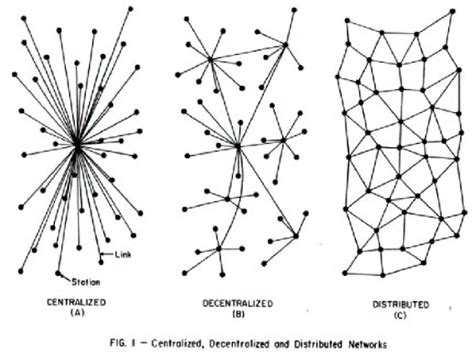
\includegraphics[width=\linewidth]{paul-bran.jpg}
% 	\caption{An ideal case of TARA((1,-2)(1,-2)) network demonstrating TARA architecture with each service cluster suffering from two byzantine / non-byzantine faults.}
% 	\label{fig:3.4}
% \end{figure}

\section{Applicability}
\subsection{Sentinel Scalability}
\subsection{Modulated Trust}
\subsection{Throughput}

\section{Implementation and evaluation}
\subsection{Reference implementation}
The implementation of the proposed architecture doesn’t require special care or teaching, but needs the practical approach to implementing its technique showcased to drastically reduce the rate of absolute system failure. 

We encourage the reader to contact the author, if any correspondence is required to assist/guide in implementing or evaluating the architecture on an existing BFT Raft system fulfilling the design requirements mentioned in Section 3.1.

Since Raft systems communicate through RPCs, we propose the reader to create a new RPC for nodes to communicate the point of failure and current state to the star node in case of TARA((1,-2), (1,-2)). The AppendEntries RPC[2] from leader may be extended to adding the identity of star nodes.

\subsection{Performance}

\section{Related work}
Numerous consensus algorithms have been designed, specified and implemented to address a scalable consensus for large scale internetworks such as Blockchain. Some of the algorithms are as follows:
\begin{description}
	\item[$\bullet$ Tendermint BFT] The Tendermint BFT consensus algorithm
\end{description}

\section{Conclusion}
We have proposed TARA, with various design-centric attributes and mathematical techniques that prove the liveness, safety and certainty of the distributed system. The proposed architecture not only prescribes to the theories of Practical Byzantine Fault Tolerance, Raft algorithm etc., but also improves upon the robustness of the system over failure rates, thereby making the system free of fault-prone environments and increasing availability without added cost of time and compute.

\section{Acknowledgement}
We are grateful to the authors of all the cited articles, papers and code implementations for providinginvaluable knowledge, research resources, time, guidance and feedback on the TARA architecture.

\bibliography{references.bib} 
\bibliographystyle{ieeetr}

\end{document}
